\chapter{Metodología}
\label{cap:metodologia}

\section{Herramientas de Simulación y Procesado}
\label{sec:metodologia:herramientas}

Para llevar a cabo los objetivos propuestos en este trabajo, se han utilizado diversas herramientas para los distintos procesos tanto de simulación como de procesado y análisis de datos.

\subsection{Software de simulación: \penred.}

Como ya se mencionó en la sección \ref{sec:estado_del_arte_fund_teoricos:penelope_penred}, \penred es un entorno de simulación de Monte Carlo modular, personalizable y totalmente paralelizable para el transporte de radiación en la materia. Desarrollado en C++ por \citeauthor{Gimnez-Alventosa2021}, siguiendo el estándar C++14, este software actúa como una interfaz orientada a objetos sobre el motor físico de PENELOPE, heredando sus modelos de interacción y algoritmos de transporte de partículas.

Su arquitectura destaca por implementar un doble enfoque de paralelismo: mediante el uso de hilos (\textit{threads}) de C++ para sistemas de memoria compartida y a través del estándar MPI (\emph{Message Passing Interface}) para infraestructuras de memoria distribuida. Gracias a su estructura modular, \penred permite extender sus funcionalidades mediante módulos de usuario sin modificar el núcleo del código. En este trabajo resulta fundamental el uso del módulo \texttt{PENNUC}, el cual permite la simulación de esquemas de desintegración nuclear complejos que no están disponibles en los generadores de eventos estándar de PENELOPE, permitiendo modelar con precisión el decaimiento del \yochoseis.

\subsubsection{Definiciones Clave de la Simulación}

Para una correcta comprensión de los resultados obtenidos y del funcionamiento del flujo de trabajo, es necesario establecer una serie de definiciones fundamentales dentro del ecosistema de \penred:

\begin{itemize}
  \item \textbf{Partículas Primarias y Secundarias:} Las partículas primarias son aquellas generadas directamente por la fuente (por ejemplo, el positrón y los \textit{prompt gammas} en el $^{86}\text{Y}$). Las secundarias son producidas por interacciones de otras partículas, como los fotones de \SI{511}{\kilo\electronvolt} resultantes de la aniquilación del positrón.
  \item \textbf{Historia (\textit{History}):} Representa la unidad básica de simulación. Una historia comprende una partícula primaria (generada directamente por la fuente radiactiva) y todas las partículas secundarias derivadas de sus interacciones hasta que son absorbidas o escapan del sistema (véase un ejemplo de las trayectorias de partículas simuladas en la Figura \ref{fig:particle_track}). En este trabajo, cada historia se identifica unívocamente con un evento de desintegración, con su correspondiente número de historia.
  \item \textbf{Estado de la partícula (\textit{Particle State}):} En una simulación, \penred almacena información detallada del estado de cada partícula. Parámetros cruciales para este trabajo incluyen:
        \begin{itemize}
          \item \textbf{Edad (\textit{Age}):} El tiempo de vuelo de la partícula desde su generación. Es el parámetro crítico para evaluar la coincidencia temporal durante el post-procesado.
          \item \textbf{Geometría:} Los índices de cuerpo (\texttt{IBODY}) y material (\texttt{MAT}), que permiten identificar si una interacción ocurrió dentro de un cristal detector o en el tejido del paciente (posible \textit{scatter}).
        \end{itemize}
  \item \textbf{Etiquetas ILB e Índices de Interacción:} Para cada partícula, \penred asigna etiquetas (\textit{ILBs}) que rastrean su genealogía (índice de la partícula padre) y el mecanismo de interacción que la generó (por ejemplo, \texttt{BETAp ANNIHILATION} para la aniquilación, o \texttt{GAMMA COMPTON} para la dispersión Compton). Esta trazabilidad es el núcleo que sustenta la clasificación analítica de eventos verdaderos y falsos en los datos simulados.
  \item \textbf{\textit{Tallies}:} Los \textit{tallies} son los módulos encargados de registrar magnitudes físicas durante la simulación. En este proyecto se utiliza el \texttt{Tally Singles}. Para cada interacción en los detectores, se registra un evento guardando el estado completo de la partícula (energía depositada, \textit{Age}, posición, e identificador de historia, además de las mencionadas etiquetas ILB).
  \item \textbf{\textit{Singles}:} Se denomina \textit{single} a cualquier evento de detección individual registrado por el \texttt{Tally Singles}. Este constituye el dato crudo u \textit{output} directo de \penred.
\end{itemize}

\begin{figure}
  \centering
  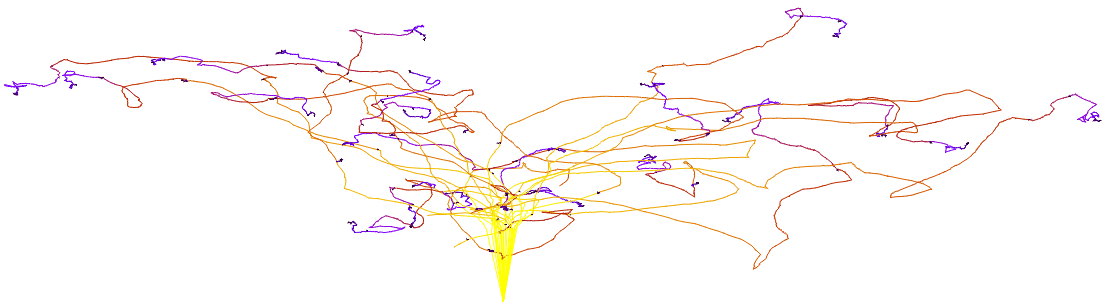
\includegraphics[width=0.9\textwidth]{figuras/particle_track.png}
  \caption{Ejemplo de la trayectoria de electrones en un medio acuoso. El color muestra el cambio en la energía del electrón. Fuente: Manual de Usuario de PenRed \cite{gimenez2025penred}.}
  \label{fig:particle_track}
\end{figure}

\subsubsection{Unidades y Constantes en \penred}

Internamente, el software opera con un sistema de unidades consistente: la longitud se mide en centímetros (cm), la energía en electronvoltios (eV), el tiempo en segundos (s) y la densidad en g/cm$^3$.

\subsubsection{Tally Singles}

El \textit{output} directo de la simulación se registra en formato binario mediante el módulo \texttt{Tally Singles}. Cada interacción válida en los detectores produce un registro individual con la siguiente estructura de memoria:

\begin{lstlisting}[language=C++, caption={Estructura de memoria de un evento individual (\textit{single}) generado por \penred.}, label={lst:single_struct}]
struct Single {
    float E;
    float x;
    float y;
    float z;
    double t;
    uint64_t hist; 
    padding[7];
};
\end{lstlisting}

En la Tabla \ref{tab:single_offset} se detalla el mapa de memoria de la estructura, cuyo tamaño total por evento es de exactamente 39 bytes.

\begin{table}[h]
  \centering
  \renewcommand{\arraystretch}{1.2}
  \begin{tabular}{c l l l}
    \hline
    \textbf{Offset} & \textbf{Campo}   & \textbf{Tipo}    & \textbf{Valor}                           \\
    \hline
    0               & \texttt{E}       & \texttt{float}   & Energía depositada (eV)                  \\
    4               & \texttt{x}       & \texttt{float}   & Coordenada espacial X (cm)               \\
    8               & \texttt{y}       & \texttt{float}   & Coordenada espacial Y (cm)               \\
    12              & \texttt{z}       & \texttt{float}   & Coordenada espacial Z (cm)               \\
    16              & \texttt{t}       & \texttt{double}  & Tiempo de vuelo o \textit{Age} (s)       \\
    24              & \texttt{hist}    & \texttt{u64}     & Identificador único de la historia       \\
    32              & \texttt{padding} & \texttt{byte[7]} & Datos adicionales ignorados\footnotemark \\
    \hline
  \end{tabular}
  \caption{Mapa de memoria y desplazamientos (\textit{offsets}) de la estructura \texttt{Single} empleada en el post-procesado.}
  \label{tab:single_offset}
\end{table}
\footnotetext{En la salida original de \penred, estos 7 bytes se corresponden con metadatos adicionales que no son requeridos en este procesado: el peso estadístico de la partícula (4 bytes), una máscara booleana de estado (1 byte), el tipo de partícula (1 byte) y el tipo de la última interacción (1 byte).}

\subsubsection{Plugin de \penred para Blender}

La definición manual de geometrías complejas mediante archivos de texto mediante superficies cuádricas tiene una complejidad asociada. A medida que aumenta la complejidad del modelo, el proceso de construcción de la geometría se vuelve más difícil, tedioso, requiere más tiempo y es propenso a errores \cite{Wilson2010}. Para superar esta limitación, en este trabajo se ha utilizado el software de modelado 3D de código abierto Blender, integrado con el plugin específico de \penred \cite{PenredBlender}.

Esta herramienta permite:
\begin{itemize}
  \item \textbf{Modelado Visual:} Construir y visualizar en 3D los volúmenes del escáner y del fantoma, asegurando la correcta alineación y evitando solapamientos físicos imposibles (\textit{overlaps}) entre los materiales.
  \item \textbf{Asignación de Materiales:} Vincular directamente los objetos 3D con los archivos de materiales de la simulación (\texttt{.mat}) y definir sus propiedades (detectores sensibles, blindajes, fantomas).
  \item \textbf{Exportación Automática:} El plugin traduce los objetos de la escena de Blender al formato de archivo de geometría (\texttt{.geo}) basado en cuádricas que utiliza \penred de forma automática y transparente al usuario.
\end{itemize}

\begin{figure}[htbp]
  \centering
  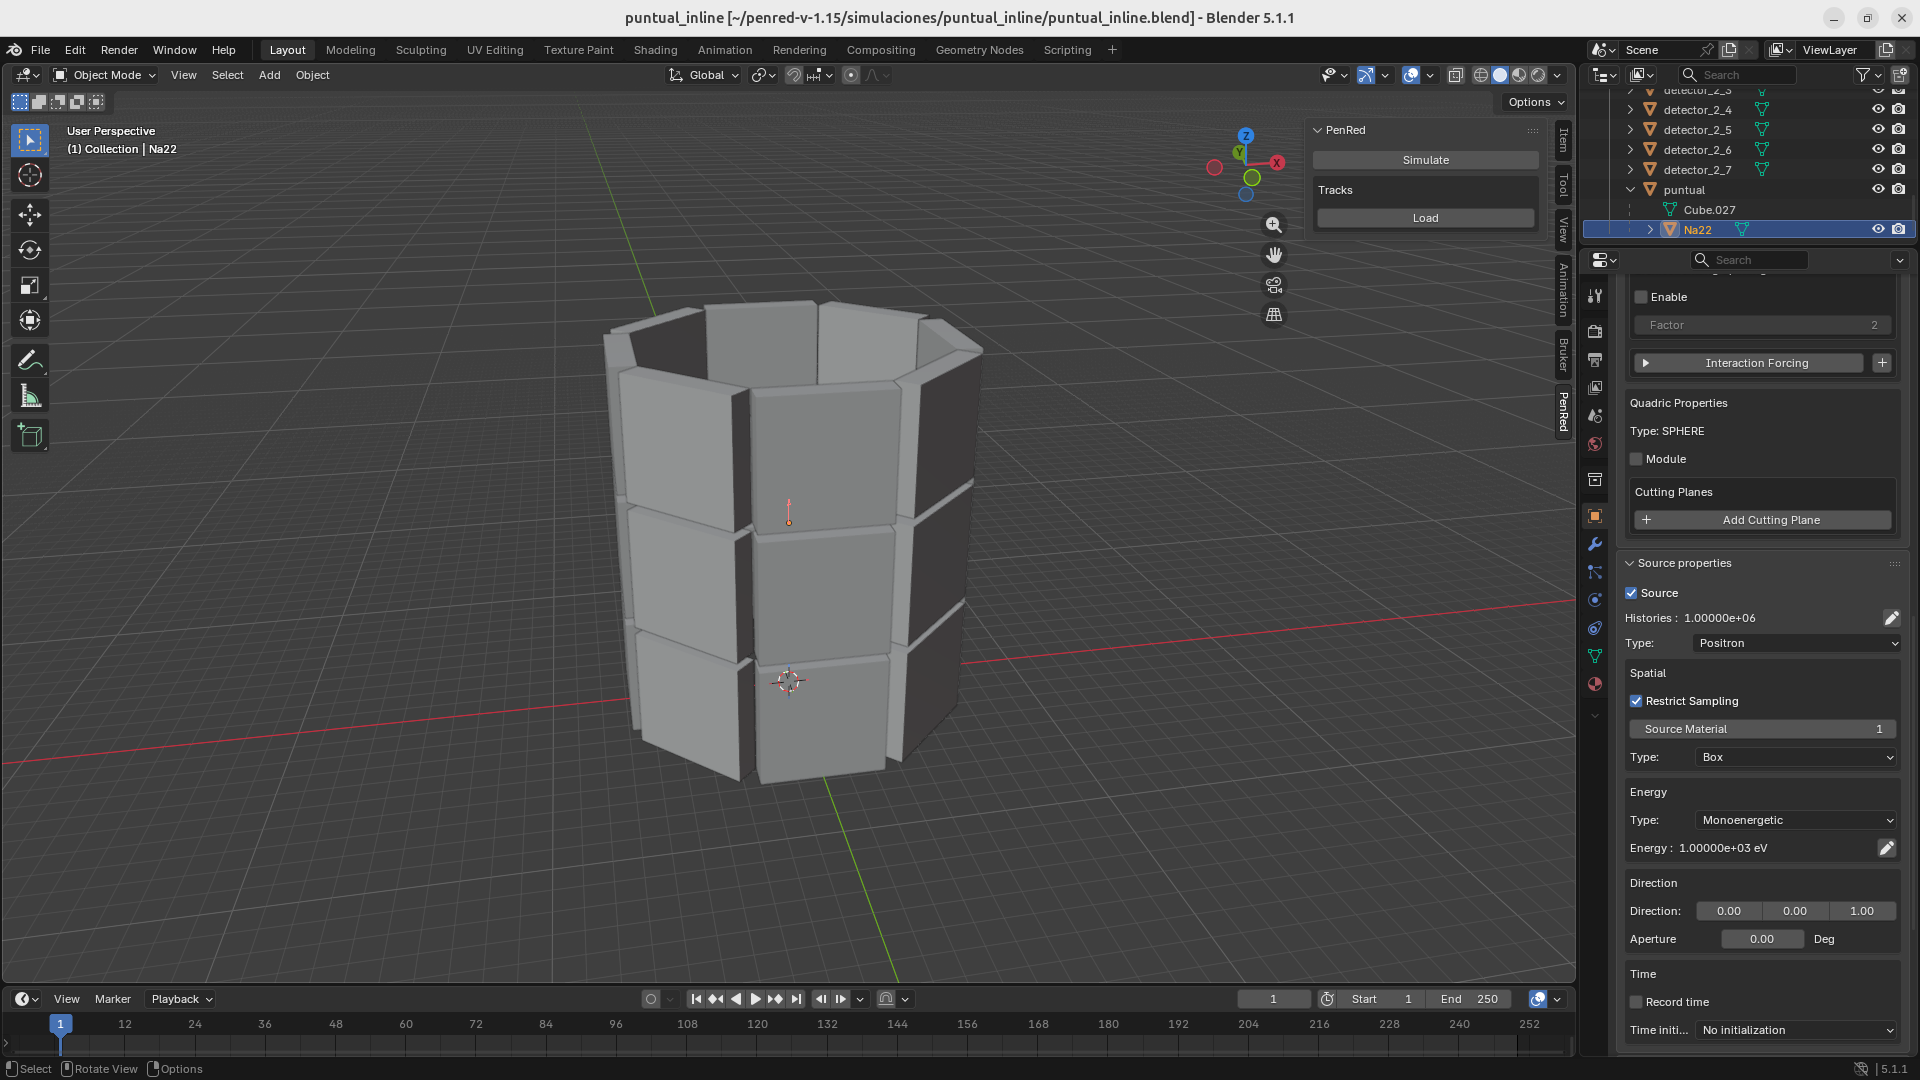
\includegraphics[width=0.90\textwidth]{figuras/blender.png}
  \caption{Interfaz del entorno de modelado Blender utilizando el plugin específico de \penred. A través de este complemento, es posible diseñar las geometrías y asignar los materiales directamente sobre el modelo 3D \cite{PenredBlender}.}
  \label{fig:blender_plugin}
\end{figure}

Gracias a este flujo de trabajo, se han podido generar modelos de alta fidelidad del escáner y el fantoma, como se muestra en la figura \ref{fig:modelos_3d}.

\subsection{Entorno de simulación: Cluster Quasar (ISIRYM)}

Las simulaciones de Monte Carlo se han ejecutado, mediante conexión remota vía SSH, en el clúster de computación de alto rendimiento Quasar, perteneciente al Instituto de Seguridad Industrial, Radiofísica y Medioambiental (ISIRYM) de la Universitat Politècnica de València. Este entorno proporciona la capacidad de cómputo necesaria para gestionar el elevado número de historias requerido para obtener estadísticas significativas en tiempos de ejecución razonables, ya que permite realizar simulaciones en paralelo.

La infraestructura técnica del clúster Quasar consta de un total de 182 núcleos de procesamiento distribuidos en 6 nodos de arquitectura AMD (5 nodos de 32 núcleos y 1 nodo de 24 núcleos). En lo referente a la memoria, cinco de estos nodos están equipados con 128 GB de RAM, mientras que el nodo restante dispone de 512 GB de RAM. Además, el sistema cuenta con una capacidad de almacenamiento de 33 TB. Esta configuración de altas prestaciones resulta idónea para optimizar los recursos en las tareas de paralelización masiva mediante MPI y \textit{threads} que requiere \penred.

\subsection{Software de reconstrucción: Bruker RecoServer (Algoritmo MLEM).}

Los sistemas PET preclínicos de Bruker incorporan una cadena de reconstrucción de imagen dedicada, diseñada para procesar los datos adquiridos por el escáner. El componente central de este flujo de trabajo es el \texttt{RecoServer}, un módulo responsable de transformar los eventos de coincidencia en distribuciones volumétricas de actividad mediante algoritmos de reconstrucción iterativa.

La reconstrucción se fundamenta en el MLEM (ver sección \ref{subsubsec:mlem}), el cual resulta idóneo para la tomografía por emisión de positrones debido a su capacidad para modelar la naturaleza estadística de Poisson del decaimiento radiactivo y la detección. El MLEM actualiza la imagen de forma iterativa comparando las proyecciones medidas con las predichas por la estimación actual de la imagen, ajustando la intensidad de los vóxeles para maximizar la verosimilitud de los datos observados.

La implementación de Bruker incluye opciones para correcciones físicas como la atenuación, la dispersión (\textit{scatter}) y las coincidencias aleatorias (\textit{randoms}), entre otras. Sin embargo, para aislar los efectos de las estrategias de post-procesado propuestas en este trabajo (ventanas de energía y tiempo), se desactivaron deliberadamente todas las correcciones del software de reconstrucción. De este modo, cualquier variación en la calidad de imagen final es atribuible exclusivamente a los cambios en los datos de entrada (\textit{input data}) y no al algoritmo de reconstrucción.

La configuración de reconstrucción empleada en este estudio se resume en la Tabla \ref{tab:reco_params}. Se mantuvo idéntica para todas las fases experimentales (desde la ideal hasta la optimizada).

\begin{table}[h]
  \centering
  \renewcommand{\arraystretch}{1.3}
  \begin{tabular}{l l}
    \hline
    \textbf{Parámetro}       & \textbf{Valor}                       \\
    \hline
    Algoritmo                & MLEM                                 \\
    Iteraciones              & 16                                   \\
    Subsets                  & 1                                    \\
    Matriz de reconstrucción & $180 \times 180 \times 300$ vóxeles  \\
    Tamaño de vóxel          & \SI{0.50}{\milli\meter} (isotrópico) \\
    \hline
    Scatter                  & 0 (desactivado)                      \\
    Randoms                  & 0 (desactivado)                      \\
    Atenuación               & None (desactivada)                   \\
    PSF                      & 1.0                                  \\
    \hline
  \end{tabular}
  \caption{Parámetros de reconstrucción del \texttt{RecoServer} utilizados en todas las fases del estudio.}
  \label{tab:reco_params}
\end{table}

La discretización espacial de \SI{0.50}{\milli\meter} permite una resolución suficiente para resolver las varillas más finas del fantoma Derenzo sin comprometer excesivamente la estadística por vóxel.

\subsection{Análisis de imagen: AMIDE.}
% rois y obtención de la intensidad
Para la visualización, manipulación y extracción de datos cuantitativos de los volúmenes reconstruidos, se ha utilizado el software AMIDE (\textit{A Medical Image Data Examiner}). Se trata de una herramienta de código abierto multiplataforma diseñada específicamente para el análisis de imagen molecular volumétrica (PET, SPECT, CT).

En el contexto de este trabajo, AMIDE ha desempeñado dos funciones fundamentales: la inspección cualitativa visual y la cuantificación numérica mediante Regiones de Interés (ROIs). La interfaz principal de este software se muestra en la Figura \ref{fig:interfaz_amide}.

\begin{figure}[htbp]
  \centering
  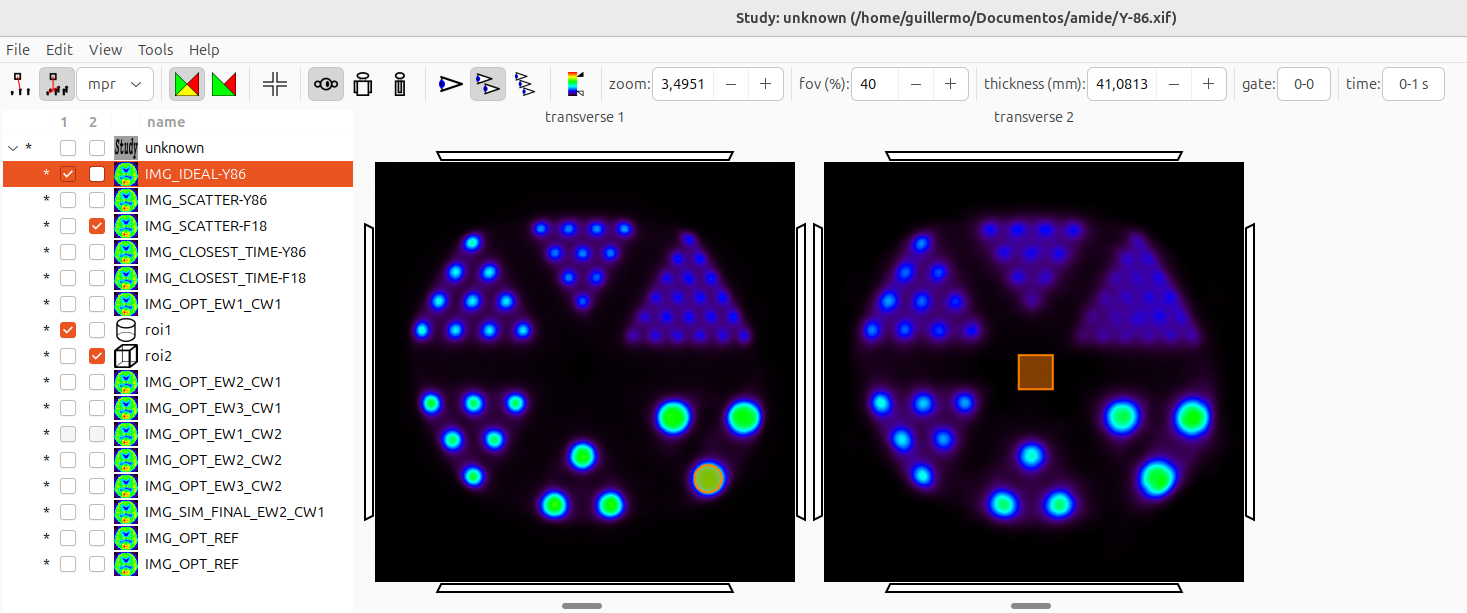
\includegraphics[width=0.9\textwidth]{figuras/interfaz_amide.png}
  \caption{Interfaz principal del software AMIDE (\textit{A Medical Image Data Examiner}), utilizado para la visualización y análisis cuantitativo de los volúmenes reconstruidos.}
  \label{fig:interfaz_amide}
\end{figure}

\subsubsection{Definición de Regiones de Interés (ROIs)}

Para evaluar la calidad de la imagen y calcular las métricas de desempeño, es necesario medir la concentración de actividad en zonas específicas del fantoma. Dada la geometría del fantoma Derenzo (formado por varillas cilíndricas), se ha seguido la siguiente metodología:

\begin{enumerate}
  \item \textbf{Selección de Geometría:} Se han utilizado ROIs volumétricas de tipo Cilindro Elíptico (\textit{Elliptic Cylinder}). Esta geometría se ajusta óptimamente a la forma física de las varillas del fantoma, minimizando la inclusión de vóxeles de borde que podrían introducir errores por volumen parcial.
  \item \textbf{Estrategia de Posicionamiento Consistente:} Para garantizar que las comparaciones entre diferentes simulaciones (Ideal vs. Realista vs. Optimizada) sean científicamente válidas, se ha aplicado el siguiente protocolo:
        \begin{itemize}
          \item Las ROIs se dibujaron inicialmente sobre la imagen de la Simulación Ideal (\texttt{SIM\_IDEAL}), donde la ausencia de ruido y la nitidez de los bordes permiten un posicionamiento perfecto sobre las varillas calientes y el fondo.
          \item Una vez definido el conjunto de ROIs (varillas de distintos diámetros y región de fondo), este se copió y aplicó exactamente en las mismas coordenadas espaciales a todas las demás imágenes reconstruidas. Esto asegura que las variaciones medidas se deben exclusivamente a los efectos físicos y de procesado, y no a errores manuales de delimitación.
        \end{itemize}
  \item \textbf{Regiones Definidas:}
        \begin{itemize}
          \item \textbf{ROIs Calientes ($ROI_{hot}$):} Se definieron cilindros individuales sobre las varillas de los seis sectores del fantoma (\SI{0.8}{\milli\meter} a \SI{2.5}{\milli\meter}) para evaluar la recuperación del contraste en función del tamaño.
          \item \textbf{ROI de Fondo ($ROI_{bkg}$):} Se definió una región cilíndrica de gran volumen en una zona uniforme del fantoma, alejada de las varillas activas, para caracterizar el ruido de fondo.
        \end{itemize}
\end{enumerate}

La disposición y el ajuste de estas ROIs cilíndricas sobre los sectores activos del fantoma Derenzo en el entorno de AMIDE se ilustran en la Figura \ref{fig:roi_amide}.

\begin{figure}[htbp]
  \centering
  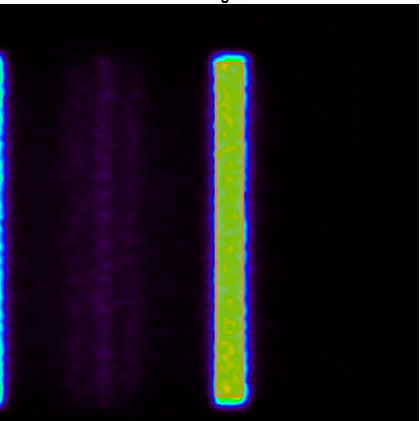
\includegraphics[width=0.85\textwidth]{figuras/roi_amide.png}
  \caption{Definición de las Regiones de Interés (ROIs) cilíndricas sobre la imagen reconstruida de la simulación ideal del fantoma Derenzo en el entorno de AMIDE.}
  \label{fig:roi_amide}
\end{figure}

\subsubsection{Obtención de la Intensidad y Estadística}

Para cada ROI definida, AMIDE calcula estadísticas sobre los valores de los vóxeles contenidos en ella. Para este estudio, se han extraído los siguientes parámetros:

\begin{itemize}
  \item \textbf{Media ($\mu$):} Valor promedio de intensidad en la ROI. Utilizado como estimador de la señal para el cálculo del CRC.
  \item \textbf{Desviación Estándar ($\sigma$):} Medida de la dispersión de los valores de los vóxeles dentro de la ROI. Utilizada fundamentalmente en la ROI de fondo para calcular el ruido y determinar la SNR.
\end{itemize}

Los datos estadísticos crudos exportados de AMIDE se procesaron posteriormente en hojas de cálculo para aplicar las fórmulas de las métricas de calidad descritas en la sección \ref{sec:metodologia:metricas}.


\section{Métricas de Evaluación de Calidad}
\label{sec:metodologia:metricas}

Para realizar una comparación objetiva entre las diferentes configuraciones de simulación y evaluar el éxito de la optimización de parámetros, es necesario definir métricas cuantitativas que caractericen la calidad de la imagen.

Basándonos en la literatura estándar de caracterización de equipos PET y en los protocolos NEMA, se han seleccionado dos indicadores fundamentales: el Coeficiente de Recuperación de Contraste (para evaluar la detectabilidad) y la Relación Señal-Ruido (para evaluar la calidad estadística).

\subsection{Coeficiente de Recuperación de Contraste (CRC).}

El contraste es la característica más crítica en la imagen oncológica, ya que determina la capacidad del sistema para distinguir una lesión tumoral (zona caliente) del tejido circundante (fondo).

El Coeficiente de Recuperación de Contraste (CRC) cuantifica la intensidad de la señal en las varillas del fantoma relativa a la actividad de fondo. Se calcula utilizando la siguiente expresión:

\begin{equation}
  CRC = \frac{\mu_{hot}}{\mu_{bkg}} - 1
  \label{eq:crc}
\end{equation}

Donde:
\begin{itemize}
  \item $\mu_{hot}$: Es la concentración media de actividad medida en la ROI de la varilla caliente (\textit{Signal}).
  \item $\mu_{bkg}$: Es la concentración media de actividad medida en la ROI de fondo (\textit{Background}).
\end{itemize}

\textbf{Interpretación en este trabajo:}
En un sistema ideal sin ruido de fondo, si el fantoma solo tiene actividad en las varillas, $\mu_{bkg}$ tendería a cero y el CRC tendería a infinito.
En el caso del $^{86}\text{Y}$, la presencia de coincidencias triples y aleatorias eleva artificialmente el valor de $\mu_{bkg}$, lo que reduce drásticamente el denominador y colapsa el valor del CRC. Por tanto, el objetivo principal de la optimización de la ventana de energía (ver sección \ref{subsec:fase4}) es reducir $\mu_{bkg}$ para maximizar el CRC.

Adicionalmente, se espera que el CRC varíe en función del diámetro de la varilla debido al Efecto de Volumen Parcial (PVE). Las varillas más pequeñas (inferiores a 2-3 veces la resolución espacial del sistema) sufrirán una pérdida de señal ($\mu_{hot}$ menor a la real) debido al vertido de cuentas (\textit{spill-out}) hacia el fondo, resultando en CRCs menores que las varillas grandes.

\subsection{Relación Señal-Ruido (SNR).}

la Relación Señal-Ruido (SNR, \textit{Signal-to-Noise Ratio}) evalúa la precisión o la \enquote{limpieza} estadística de la imagen. Un SNR alto indica una imagen suave y uniforme en zonas homogéneas, mientras que un SNR bajo indica una imagen \enquote{granulosa} o ruidosa.

Para este estudio, se ha utilizado la definición de SNR basada en la estadística de la región de fondo, calculada como:

\begin{equation}
  SNR = \frac{\mu_{bkg}}{\sigma_{bkg}}
  \label{eq:snr}
\end{equation}

Donde:
\begin{itemize}
  \item $\mu_{bkg}$: Es la concentración media en la ROI de fondo.
  \item $\sigma_{bkg}$: Es la desviación estándar de los valores de los vóxeles dentro de la misma ROI de fondo.
\end{itemize}

Esta métrica es fundamental para evaluar el coste de las estrategias de optimización. Al estrechar las ventanas de energía o tiempo para rechazar eventos espurios (mejorando el CRC), inevitablemente también se rechazan algunas coincidencias verdaderas. Esto reduce la estadística total de conteo ($N$), lo que teóricamente aumenta el ruido estadístico (el ruido Poissoniano es proporcional a $1/\sqrt{N}$).
El SNR permite monitorizar si la estrategia de limpieza de imagen mantiene una calidad estadística aceptable para el diagnóstico.

\section{Definición del Escenario de Simulación}
\label{sec:metodologia:escenario_sim}

Para garantizar la validez clínica de los resultados, se ha modelado un entorno de simulación que replica fielmente las condiciones de una adquisición preclínica real. Este escenario se compone de tres elementos fundamentales: la geometría del escáner, el objeto a visualizar (fantoma) y la fuente radiactiva.

\begin{figure}[htbp]
  \centering
  
\includegraphics[width=0.45\textwidth]{si78--357.png}
  \caption{Imagen comercial del escáner preclínico Bruker PET/CT Si78.}
  \label{fig:geometria_bruker}
\end{figure}

\subsection{Modelado del escáner: Geometría del Bruker PET/CT Si78.}
\label{subsec:metodologia:escenario_sim:geometria_bruker}

El sistema de detección simulado se basa en las especificaciones técnicas del escáner preclínico comercial Bruker PET/CT Si78. La geometría se ha definido en Blender y se ha exportado a geometría constructiva de cuádricas (\texttt{PEN\_QUADRIC}) gracias al plugin para Blender de \penred.

El modelo virtual consta de un tres anillos de detectores con las siguientes características:

\begin{itemize}
  \item \textbf{Configuración Geométrica:} Disposición octogonal formada por 8 módulos detectores por anillo.
  \item \textbf{Estructura Axial:} El sistema completo consta de 3 anillos contiguos, cubriendo un Campo de Visión (FOV) axial suficiente para albergar el fantoma completo.
  \item \textbf{Dimensiones del Módulo:} Cada bloque detector tiene unas dimensiones de superficie activa de $\SI{48.0}{\milli\meter} \times \SI{48.0}{\milli\meter}$ y un espesor de cristal de $\SI{10.0}{\milli\meter}$.
  \item \textbf{Diámetro del Escáner:} La distancia entre detectores opuestos se ha fijado en $\SI{117.0}{\milli\meter}$.
  \item \textbf{Material del Centelleador:} Se ha asignado al volumen sensible las propiedades físicas del LYSO (Lutecio-Itrio Oxiortosilicato), definiendo su densidad ($\rho = \SI{7.1}{\gram\per\cubic\centi\meter}$) y composición elemental para simular correctamente la atenuación y la eficiencia de detección de los fotones de \SI{511}{\kilo\electronvolt} y los \emph{prompt gammas}.
\end{itemize}

\begin{figure}[htbp]
  \centering
  \begin{subfigure}[b]{0.45\textwidth}
    \centering
    
\includegraphics[width=\textwidth]{pet_geo.png}
    \caption{Modelo 3D del escáner Bruker Si78.}
  \end{subfigure}
  \hfill
  \begin{subfigure}[b]{0.45\textwidth}
    \centering
    
\includegraphics[width=\textwidth]{derenzo.png}
    \caption{Modelo 3D del fantoma Derenzo.}
  \end{subfigure}

  \vspace{0.5cm}

  \begin{subfigure}[b]{0.45\textwidth}
    \centering
    
\includegraphics[width=\textwidth]{geometria_completa2.png}
    \caption{Modelo 3D del fantoma Derenzo situado dentro del escáner.}
  \end{subfigure}
  \caption{Visualización en Blender de las geometrías modeladas para la simulación. El plugin de \penred permite exportar estos modelos directamente al archivo de configuración de la simulación.}
  \label{fig:modelos_3d}
\end{figure}

Esta configuración permite reproducir efectos geométricos realistas, como la variación de la sensibilidad en el FOV y las pérdidas por espacios muertos (\emph{gaps}) entre módulos.

\subsection{El Fantoma Derenzo: Especificaciones y materiales.}

Para evaluar la resolución espacial y el contraste, se ha utilizado un modelo digital del Fantoma de Calidad de Imagen (IQ) tipo Derenzo. El fantoma consiste en un cilindro de PMMA (Poli-metacrilato de metilo) de $\SI{35}{\milli\meter}$ de radio, que contiene perforaciones cilíndricas (varillas) de $\SI{10}{\centi\meter}$ de largo que se rellenan con la disolución radiactiva. Las varillas están agrupadas en seis sectores, variando su diámetro para evaluar distintos niveles de resolución espacial.

Los diámetros de las varillas simuladas son:
\begin{itemize}
  \item $\SI{0.8}{\milli\meter}$, $\SI{1.0}{\milli\meter}$, $\SI{1.2}{\milli\meter}$, $\SI{1.5}{\milli\meter}$, $\SI{2.0}{\milli\meter}$ y $\SI{2.5}{\milli\meter}$.
\end{itemize}

La distancia entre los centros de las varillas en cada sector es igual al doble de su diámetro, lo que permite evaluar la capacidad del sistema para separar fuentes puntuales cercanas.

En cuanto a los materiales, se han definido dos configuraciones para las distintas fases del estudio:
\begin{enumerate}
  \item \textbf{Configuración Ideal:} Tanto el cuerpo del fantoma como las varillas se definen como \enquote{vacío} (\texttt{void.mat}) para eliminar la atenuación y el \emph{scatter}.
  \item \textbf{Configuración Realista:} Tanto el cuerpo del fantoma (material de atenuación) como las varillas activas se han definido como \enquote{agua} (\texttt{water.mat}). Esto simula un entorno de dispersión y atenuación equivalente a tejido blando, siendo una aproximación estándar en física médica.
\end{enumerate}

\subsection{Configuración de la fuente radiactiva (Archivos .nuc).}

La fuente radiactiva se ha simulado utilizando el módulo PENNUC de \penred, el cual requiere archivos de datos nucleares (\texttt{.nuc}) que describen el esquema de desintegración completo.

Estos archivos se han generado a partir de los datos obtenidos de la base de datos de referencia NuDat 3 del National Nuclear Data Center \parencite{bnlNuDat}. Se han empleado dos archivos:

\begin{itemize}
  \item \textbf{\texttt{F18.nuc}:} Simula el decaimiento del $^{18}\text{F}$, generando pares de aniquilación puros como referencia.
  \item \textbf{\texttt{Y86.nuc}:} Simula el decaimiento complejo del $^{86}\text{Y}$ con sus probabilidades de ramificación correctas. Gracias a los datos de NuDat 3, este archivo incluye el espectro completo de \emph{prompt gammas} (ej. \SI{1077}{\kilo\electronvolt}, \SI{628}{\kilo\electronvolt}) emitidos en coincidencia con el positrón, permitiendo la simulación realista de coincidencias triples.
\end{itemize}



\section{Algoritmo de Post-Procesado (C++)}
\label{sec:metodologia:postprocess}

La simulación Monte Carlo con \texttt{penRed} genera como salida archivos de datos en modo lista que contienen eventos individuales o \textit{singles}. Cada entrada registra la posición, el tiempo, la energía depositada y, crucialmente para la validación, el identificador de la historia (\textit{EventID}) de cada interacción en el detector.

Para reconstruir imágenes PET, es necesario procesar estos eventos individuales para identificar pares de fotones que correspondan a una aniquilación. Dado que este proceso requiere una lógica específica no disponible en las herramientas de reconstrucción estándar, se ha utilizado un software de post-procesado escrito en C++

La base del código de post-procesado (\texttt{createCoincidences}) es una herramienta de investigación interna desarrollada en Bruker. Sobre esta arquitectura base, en el marco de este TFG, se han desarrollado e implementado extensiones específicas para incorporar la lógica de detección de triples y separación de isótopos (Multiplexing), adaptando la metodología descrita en la literatura \parencite{Andreyev2011}.

\subsection{Arquitectura y flujo de datos.}

La arquitectura del software sigue un modelo de procesamiento secuencial basado en ventanas de tiempo, optimizado para manejar eficientemente grandes volúmenes de datos provenientes de múltiples módulos detectores. El flujo de ejecución se estructura en las siguientes etapas:

\begin{enumerate}
  \item \textbf{Entrada y Configuración:}
        El programa lee un archivo de configuración que define la geometría del escáner (tamaño de detectores, anillos, módulos), parámetros físicos del isótopo y la configuración de la adquisición. Además, carga una lista de pares permitidos (\texttt{detectorList.txt}) que define qué módulos detectores están en coincidencia geométrica válida (\textit{Field of View}). Los datos de eventos individuales (\textit{singles}) se leen desde archivos binarios separados (\texttt{.dat}), uno por cada módulo detector.
  \item \textbf{Gestión de Buffer Temporal:}
        Para evitar cargar la totalidad de los datos en memoria, el programa utiliza un búfer dinámico (\texttt{nextSingles}). El sistema carga iterativamente eventos de todos los archivos de módulo, manteniéndolos ordenados cronológicamente. Se define una ventana de tiempo de coincidencia (\textit{coincidenceWindow}) y, en cada iteración, el programa analiza los eventos dentro de esta ventana deslizante para identificar pares válidos, descartando los eventos antiguos una vez procesados.
  \item \textbf{Modelado de la Respuesta del Detector (\textit{Energy Blurring}):}
        Dado que la simulación Monte Carlo registra la energía depositada exacta ($E_{dep}$), el post-procesado es responsable de introducir el modelado realista de la resolución energética. Esta funcionalidad se implementa en la función de lectura \texttt{readPenRed}. Para cada evento individual, se aplica un desenfoque gaussiano basado en la resolución energética ($R_E$, definida como FWHM a \SI{511}{\kilo\electronvolt}). La desviación estándar $\sigma$ se calcula como:

        \begin{equation}
          \sigma = \frac{E_{dep} \cdot R_E}{2.355}
        \end{equation}
        y se suma un valor aleatorio de una distribución normal $\mathcal{N}(0, \sigma)$ a la energía original. Este paso es fundamental para simular la respuesta real del cristal centelleador y evaluar el rechazo de eventos dispersos (\textit{scatter}). En este trabajo, se estableció una resolución energética del 14\% (FWHM a \SI{511}{\kilo\electronvolt}) y una resolución espacial intrínseca de \SI{0.08}{cm}, valores típicos para este tipo de escáner.

  \item \textbf{Salida:}
        Los eventos de coincidencia identificados se proyectan sobre la superficie de los detectores y se escriben en formato List-Mode (LM).
\end{enumerate}

\subsection{Algoritmos de coincidencia:}

El núcleo del programa evalúa los eventos en el búfer temporal para formar pares. El algoritmo toma el evento más antiguo del búfer (evento de referencia) y busca una pareja entre los siguientes eventos que cumpla dos condiciones básicas: estar dentro de la ventana de coincidencia temporal y pertenecer a un módulo detector opuesto válido.
Se han utilizado tres modos distintos para cubrir las diferentes fases del estudio. Mientras que los dos primeros ya estaban presentes en la implementación original de Bruker, el tercero (multiplexado) ha sido desarrollado íntegramente en este trabajo:

\textbf{Modo Ideal (\textit{Take Same History})}: Este modo, activado con el flag \texttt{TAKE\_SAME\_HISTORY}, aprovecha la información \enquote{ground truth} de la simulación Monte Carlo para validación. Cada evento registrado por penRed incluye un identificador único de la desintegración original (\textit{EventID} o historia). El algoritmo busca un segundo evento que tenga exactamente el mismo identificador de historia (\texttt{hist}) que el evento de referencia. Permite separar coincidencias \enquote{verdaderas} ideales de cualquier coincidencia aleatoria (\textit{random}) o espuria. Es esencial para validar la geometría y la normalización en condiciones ideales (\ref{subsec:fase1} y \ref{subsec:fase2}).

\begin{lstlisting}[language=C++, caption={Implementación de la lógica de detección basada en tomar como pareja solo si proviene de la misma historia.}, label={lst:take_closest}]
	case COINCIDENCE_METHOD::TAKE_SAME_HISTORY:

      for (size_t i = 1; i < nextSingles.size(); ++i) {
        // Get pair
        localPair = getPair(pairIndexes, nextSingDevMod,
                            sim2devModule(modPerRing, nextSingles[i].module));
        if (localPair >= pairIndexes.size())
          continue;

        // Check if can be considered as the next coincidence
        if (hist == nextSingles[i].hist) {
          iCoincidence = i;
          iPair = localPair;
          break;
        }
      }
	  break;
\end{lstlisting}

\textbf{Modo Realista (\textit{Take Closest})}: Este modo se activa con el flag \texttt{TAKE\_CLOSEST}, emula el comportamiento de la electrónica de coincidencias de un escáner PET real. Dado que el búfer de eventos está ordenado temporalmente, el algoritmo selecciona como pareja al primer evento válido que encuentra en el búfer (que cumpla los criterios de energía y geometría). Al estar ordenados por tiempo, este evento es intrínsecamente el que tiene la menor diferencia de tiempo ($\Delta t$) con respecto al evento de referencia. Es el modo estándar para generar datos realistas (secciones \ref{subsec:fase3} y \ref{subsec:fase4}). Introduce naturalmente coincidencias aleatorias (\textit{randoms}) si la tasa de cuentas es alta, tal como ocurriría en un detector físico.

\begin{lstlisting}[language=C++, caption={Implementación de la lógica de detección basada en tomar el primer evento válido dentro de la ventana de coincidencia.}, label={lst:take_closest}]
	case COINCIDENCE_METHOD::TAKE_CLOSEST:
    default:
      for (size_t i = 1; i < nextSingles.size(); ++i) {
        // Get pair
        localPair = getPair(pairIndexes, nextSingDevMod,
                            sim2devModule(modPerRing, nextSingles[i].module));
        if (localPair >= pairIndexes.size())
          continue;

        iCoincidence = i;
        iPair = localPair;
        break;
      }
      break;
\end{lstlisting}

\textbf{Modo Multiplexado (\textit{Take Closest Multiplexing})}: Este modo avanzado, activado con el flag \texttt{TAKE\_CLOSEST\_MULTIPLEXING}, está diseñado específicamente para simulaciones con isótopos emisores de gammas rápidos en cascada, permitiendo la detección de coincidencias triples (sección \ref{subsec:fase5}).

\begin{lstlisting}[language=C++, caption={Implementación de la lógica de detección de eventos triples (Multiplexing).}, label={lst:triple_logic}]
    case COINCIDENCE_METHOD::TAKE_CLOSEST_MULTIPLEXING:
      for (size_t i = 1; i < nextSingles.size(); ++i) {
        localPair = getPair(pairIndexes, nextSingDevMod,
                            sim2devModule(modPerRing, nextSingles[i].module));
        if (localPair >= pairIndexes.size())
          continue;

        // Filter standard singles by emax (ensure they are 511 candidates)
        if (nextSingles[i].e > emax)
          continue;

        // Found the valid pair (Closest in time)
        iCoincidence = i;
        iPair = localPair;

        // Scan for Prompt Gamma (Triple) anywhere in the current buffer
        for (size_t k = 0; k < nextSingles.size(); ++k) {
          if (k == 0 || k == i)
            continue;
          if (nextSingles[k].e >= promptGammaThreshold) {
            isTriple = true;
            break;
          }
        }
        break;
      }
      break;
\end{lstlisting}

\begin{itemize}
  \item \textbf{Lectura Ampliada:} A diferencia de los otros modos, se cargan eventos en un rango de energía extendido que incluye tanto los fotones de aniquilación (\SI{511}{\kilo\electronvolt}) como los gammas de alta energía (\textit{prompt gammas}, hasta \texttt{promptGammaMax}).
  \item \textbf{Identificación de Par PET:} Primero, el algoritmo busca una coincidencia estándar tipo \textit{Closest Time}, restringiendo la búsqueda de la pareja a la ventana de energía de \SI{511}{\kilo\electronvolt} (\texttt{energy <= emax}) para definir la Línea de Respuesta (LOR).
  \item \textbf{Detección de Triple:} Una vez encontrado un par PET válido, el algoritmo escanea el búfer actual en busca de un tercer evento (en cualquier posición temporal relativa válida) cuya energía supere el umbral de gammas rápidos (\texttt{promptGammaThreshold}).
  \item \textbf{Salida Dual:} El software genera dos archivos de salida:
        \begin{itemize}
          \item \texttt{data\_AB.lm}: Contiene todas las coincidencias detectadas (para reconstrucción estándar de la mezcla).
          \item \texttt{data\_B\_prime.lm}: Contiene exclusivamente aquellas coincidencias donde se detectó el tercer gamma (triple), lo que permite estudiar técnicas de reconstrucción multiplexada para la separación de isótopos.
        \end{itemize}
\end{itemize}

\begin{lstlisting}[language=C++, caption={Escritura condicional de los archivos de salida para la separación de isótopos.}, label={lst:writing_logic}]
// Save bruker format
    if (outputFormat != OUTPUT_FORMAT::CASTOR) {
      if (outputFormat != OUTPUT_FORMAT::BRUKER_LM_ONLY_COINCIDENCES ||
          acceptedCoincidence) {
        if (fLM != nullptr)
          fwrite(&c, sizeof(coincidence), 1, fLM);

        if (coinMethod == COINCIDENCE_METHOD::TAKE_CLOSEST_MULTIPLEXING &&
            acceptedCoincidence) {
          // Write all doubles to A+B
          if (fLM_AB)
            fwrite(&c, sizeof(coincidence), 1, fLM_AB);

          // Write only triples to B'
          if (isTriple && fLM_B_prime)
            fwrite(&c, sizeof(coincidence), 1, fLM_B_prime);
        }
      }
    }
\end{lstlisting}

En el Anejo \ref{anx:codigo} se incluyen fragmentos de código y se detalla con mayor profundidad el funcionamiento técnico de estos algoritmos.

\section{Diseño Experimental: Fases de Simulación}
\label{sec:metodologia:fases}

Para aislar y cuantificar los diferentes factores que degradan la imagen PET del \yochoseis, se ha diseñado una metodología experimental incremental. En lugar de simular directamente un escenario complejo, se han definido cinco fases sucesivas, añadiendo en cada una un grado más de complejidad física o de procesamiento.

Esto permite identificar qué parte de la degradación de la imagen se debe a la física fundamental del isótopo, qué parte a la interacción con el fantoma y qué parte a las limitaciones de la electrónica de detección.

\subsection{Validación Ideal (Ground Truth).}
\label{subsec:fase1}

El objetivo de esta fase es establecer la referencia absoluta o \textit{Ground Truth} del sistema. Se busca obtener una imagen que dependa exclusivamente de la geometría del escáner y de la distribución de la fuente, eliminando cualquier artefacto por interacción con la materia o ruido aleatorio.

\begin{itemize}
  \item \textbf{Configuración de Materiales:} Se definen todos los volúmenes del fantoma (varillas y cuerpo) y del entorno como vacío (\texttt{void.mat}). Esto elimina por completo la atenuación y la dispersión Compton (\textit{scatter}). Los fotones viajan en línea recta desde la emisión hasta el detector.
  \item \textbf{Configuración del Detector:} Se define el material del cristal detector como un absorbente perfecto (\texttt{eabs = \SI{1e30}{\electronvolt}}) para asegurar una eficiencia de detección del \SI{100}{\percent} sin dispersión inter-cristal.
  \item \textbf{Post-Procesado:} Se utiliza el modo \textbf{\textit{Take Same History}}. Esto garantiza que solo se reconstruyen pares de fotones que provienen de la misma desintegración nuclear, eliminando matemáticamente el 100\% de las \textbf{coincidencias aleatorias}.
\end{itemize}

Se simulan un total de $2\cdot 10^8$ historias en un tiempo de adquisición de 2 horas lo que resulta en una actividad de \SI{27.77}{\kilo\becquerel}.

\subsection{Estudio de Efectos Físicos (Scatter y Atenuación).}
\label{subsec:fase2}

En esta fase se activa la física de transporte completa en el fantoma y el detector.

\begin{itemize}
  \item \textbf{Configuración de Simulación:} Se utilizan los materiales descritos en la figura \ref{fig:materiales}: fantoma de agua, entorno de aire y detectores realistas.
  \item \textbf{Post-Procesado:} Se utiliza el modo \textbf{\textit{Take Same History}}.
\end{itemize}

Aunque la simulación incluye ahora la física completa (interacción en el agua, dispersión en el aire y respuesta intrínseca del cristal), el uso del filtro por historial en el post-procesado elimina las coincidencias aleatorias. Esto permite aislar y visualizar los efectos de la atenuación y el \textit{scatter} (tanto en el objeto como en el propio detector) antes de introducir el ruido aleatorio.


\subsection{Simulación Realista (Randoms).}
\label{subsec:fase3}

Esta fase representa la adquisición clínica real.

\begin{itemize}
  \item \textbf{Configuración de Simulación:} Se utilizan exactamente los mismos archivos de datos generados en la Fase 2 (misma configuración de materiales y fuentes). No es necesario realizar una nueva simulación Monte Carlo.
  \item \textbf{Post-Procesado:} La diferencia radica exclusivamente en el algoritmo de clasificación. Se cambia al modo \textbf{\textit{Take Closest}}.
\end{itemize}

Al ignorar la información del historial y emparejar eventos basándose únicamente en la ventana temporal ($2\tau = \SI{5}{\nano\second}$), se introducen las coincidencias aleatorias. Dado que el $^{86}\text{Y}$ genera una alta tasa de \textit{singles} debido a los \textit{prompt gammas}, y que los materiales realistas (agua/aire) generan \textit{scatter} que también contribuye a los \textit{singles}, esta fase captura la degradación máxima de la imagen: atenuación + scatter + randoms.


\subsection{ Optimización de Ventanas (Energía y Tiempo).}
\label{subsec:fase4}

Partiendo de la simulación realista, se diseñó un estudio paramétrico para determinar la configuración de adquisición que maximiza el compromiso entre contraste y ruido. El post-procesado se ejecutó iterativamente sobre los mismos datos crudos de \textit{singles}, modificando los filtros de aceptación.

Se evaluaron dos variables fundamentales:

\begin{enumerate}
  \item \textbf{Ventana de Energía (EW):} El objetivo es rechazar los fotones que han sufrido \textit{scatter} y, específicamente para el $^{86}\text{Y}$, filtrar los \textit{prompt gammas} de menor energía (como el de \SI{628}{\kilo\electronvolt}) que contaminan la ventana estándar. Se definieron tres ventanas centradas en el fotopico de \SI{511}{\kilo\electronvolt}, progresivamente más estrechas:
        \begin{itemize}
          \item \textbf{EW 20\%:} [\SI{409}{\kilo\electronvolt}, \SI{613}{\kilo\electronvolt}]
          \item \textbf{EW 15\%:} [\SI{434}{\kilo\electronvolt}, \SI{588}{\kilo\electronvolt}].
          \item \textbf{EW 10\%:} [\SI{460}{\kilo\electronvolt}, \SI{562}{\kilo\electronvolt}].
        \end{itemize}

  \item \textbf{Ventana de Coincidencia (CW):} El objetivo es reducir la tasa de coincidencias aleatorias, la cual es crítica en el $^{86}\text{Y}$. Se probaron reducciones respecto al valor estándar:
        \begin{itemize}
          \item \textbf{CW = \SI{4}{\nano\second}:}
          \item \textbf{CW = \SI{3}{\nano\second}:}
        \end{itemize}
\end{enumerate}

\subsection*{Asignación de materiales }

La asignación de materiales en la geometría de simulación se ha realizado diferenciando cuatro regiones principales —mundo, detectores, cuerpo del fantoma y varillas— y distinguiendo entre la configuración ideal (Fase 1) y la configuración realista (Fases 2-5). La Figura \ref{fig:materiales} resume esta asignación junto con la visualización gráfica correspondiente.

\begin{figure}[H]
  \centering
  % --- BLOQUE IZQUIERDO: TABLA COMPARATIVA ---
  \begin{minipage}[c]{0.58\textwidth}
    \centering
    \scriptsize % Texto un poco más pequeño para que quepa la tabla
    \renewcommand{\arraystretch}{1.5} % Más espacio entre filas
    \setlength{\tabcolsep}{3pt} % Menos espacio entre columnas

    \begin{tabular}{l | l | l}
      \hline
      \textbf{Región (Color)}                               & \textbf{Fase 1 (Ideal)}      & \textbf{Fases 2-5 (Realista)} \\
      \hline
      \textbf{Mundo} \textcolor{teal}{$\blacksquare$}       & Vacío (\texttt{void})        & Aire (\texttt{air})           \\
      \hline
      \textbf{Detectores} \textcolor{gray}{$\blacksquare$}  & \shortstack[l]{Abs. Perfecto                                 \\($E_{abs}=\SI{1e30}{eV}$)} & \shortstack[l]{LYSO\\($E_{abs}=\SI{1}{keV}$)} \\
      \hline
      \textbf{Fantoma} \textcolor{pink}{$\blacksquare$}     & Vacío (\texttt{void})        & Agua (\texttt{water})         \\
      \hline
      \textbf{Varillas} \textcolor{magenta}{$\blacksquare$} & Vacío (\texttt{void})        & Agua (\texttt{water})         \\
      \hline
    \end{tabular}
  \end{minipage}
  \hfill
  % --- BLOQUE DERECHO: VISUALIZACIÓN ---
  \begin{minipage}[c]{0.38\textwidth}
    \centering
    
\includegraphics[width=\linewidth]{materiales_colores.png}
  \end{minipage}

  \caption{Resumen de la asignación de materiales en la geometría de simulación según la fase experimental. Los colores (cuadrados) se corresponden con la visualización gráfica de la derecha. En la fase realista se introducen materiales físicos (agua, aire) y física detallada en el detector para evaluar el \textit{scatter} y la atenuación.}
  \label{fig:materiales}
\end{figure}

\subsection{ Prueba de concepto de Multiplexado.}
\label{subsec:fase5}

En esta fase final, se diseñó un experimento para validar la capacidad de separar señales de dos isótopos diferentes adquiridos simultáneamente, explotando la física de los \textit{prompt gammas}.

\textbf{Configuración del Escenario:}

Se modificó el fantoma para contener dos fuentes radiactivas distintas en regiones separadas espacialmente:

\begin{enumerate}
  \item \textbf{Ventana de Energía (EW):} El objetivo es rechazar los fotones que han sufrido \textit{scatter} y, específicamente para el $^{86}\text{Y}$, filtrar los \textit{prompt gammas} de menor energía (como el de \SI{628}{\kilo\electronvolt}) que contaminan la ventana estándar. Se definieron tres ventanas centradas en el fotopico de \SI{511}{\kilo\electronvolt}, progresivamente más estrechas:
        \begin{itemize}
          \item \textbf{EW 20\%:} [\SI{409}{\kilo\electronvolt}, \SI{613}{\kilo\electronvolt}]
          \item \textbf{EW 15\%:} [\SI{434}{\kilo\electronvolt}, \SI{588}{\kilo\electronvolt}].
          \item \textbf{EW 10\%:} [\SI{460}{\kilo\electronvolt}, \SI{562}{\kilo\electronvolt}].
        \end{itemize}

  \item \textbf{Ventana de Coincidencia (CW):} El objetivo es reducir la tasa de coincidencias aleatorias, la cual es crítica en el $^{86}\text{Y}$. Se probaron reducciones respecto al valor estándar:
        \begin{itemize}
          \item \textbf{CW = \SI{4}{\nano\second}:}
          \item \textbf{CW = \SI{3}{\nano\second}:}
        \end{itemize}
\end{enumerate}

\subsection*{Asignación de materiales }

Para esta fase, la geometría distingue cinco regiones: mundo, detectores, cuerpo del fantoma y las dos varillas activas, cada una asociada a un isótopo distinto ($^{18}\text{F}$ y $^{86}\text{Y}$). Todas las regiones emplean materiales realistas (agua, aire, LYSO), tal y como se detalla en la Figura \ref{fig:materiales_mp}.

\begin{figure}[htbp]
  \centering
  % --- BLOQUE IZQUIERDO: TABLA COMPARATIVA ---
  \begin{minipage}[c]{0.58\textwidth}
    \centering
    \scriptsize % Texto un poco más pequeño para que quepa la tabla
    \renewcommand{\arraystretch}{1.5} % Más espacio entre filas
    \setlength{\tabcolsep}{3pt} % Menos espacio entre columnas

    \begin{tabular}{l | l}
      \hline
      \textbf{Región (Color)}                                & \textbf{Material}                       \\
      \hline
      \textbf{Mundo} \textcolor{black}{$\blacksquare$}       & Aire (\texttt{air})                     \\
      \hline
      \textbf{Detectores} \textcolor{gray}{$\blacksquare$}   & \shortstack[l]{LYSO                     \\($E_{abs}=\SI{1}{keV}$)} \\
      \hline
      \textbf{Fantoma} \textcolor{blue}{$\blacksquare$}      & Agua (\texttt{water})                   \\
      \hline
      \textbf{Varilla A} \textcolor{magenta}{$\blacksquare$} & Agua (\texttt{water}) ($^{18}\text{F}$) \\
      \hline
      \textbf{Varilla B} \textcolor{pink}{$\blacksquare$}    & Agua (\texttt{water}) ($^{86}\text{Y}$) \\
      \hline
    \end{tabular}
  \end{minipage}
  \hfill
  % --- BLOQUE DERECHO: VISUALIZACIÓN ---
  \begin{minipage}[c]{0.38\textwidth}
    \centering
    
\includegraphics[width=\linewidth]{materiales_mp.png}
  \end{minipage}

  \caption{Resumen de la asignación de materiales en la geometría de simulación según la fase experimental. Los colores (cuadrados) se corresponden con la visualización gráfica de la derecha. En la fase realista se introducen materiales físicos (agua, aire) y física detallada en el detector para evaluar el \textit{scatter} y la atenuación.}
  \label{fig:materiales_mp}
\end{figure}

% \begin{figure}[hbtp]
%   \centering
%   
\includegraphics[width=0.6\textwidth]{materiales_mp.png}
%   \caption{Configuración de materiales para la prueba de concepto de multiplexado. Gris: Detectores, Azul: Agua, Negro: Aire. Las varillas centrales corresponden al isótopo limpio ($^{18}\text{F}$) y al isótopo sucio ($^{86}\text{Y}$).}
%   \label{fig:materiales_mp}
% \end{figure}

\begin{figure}[hbtp]
  \centering
  
\includegraphics[width=0.5\textwidth]{modelo_fantoma_mp.png}
  \caption{Modelo 3D del fantoma para el estudio de multiplexado.}
  \label{fig:multiplexado}
\end{figure}
\begin{itemize}
  \item \textbf{Región A:} Varilla llena exclusivamente con $^{18}\text{F}$ (isótopo puro).
  \item \textbf{Región B:} Varilla llena exclusivamente con $^{86}\text{Y}$ (isótopo sucio).
\end{itemize}

\textbf{Metodología de Separación:}
El flujo de trabajo aplicado consta de tres etapas:

\begin{enumerate}
  \item \textbf{Reconstrucción Dual:} Utilizando el modo \textit{Take Closest Multiplexing}, el post-procesado genera dos archivos de coincidencias: \texttt{data\_AB.lm} (todos los dobles) y \texttt{data\_B\_prime.lm} (solo los eventos donde se detectó un tercer gamma). Ambos se reconstruyen independientemente con el \texttt{RecoServer}, obteniéndose la imagen total ($I_{\text{total}}$) y la imagen de triples ($I_{\text{Y86}}^{\text{T}}$).
  \item \textbf{Estimación de la Contaminación:} Dado que la sensibilidad de detección de triples es mucho menor que la de dobles, la imagen $B'$ representa la distribución espacial del $^{86}\text{Y}$ pero con menor intensidad. Se asume que la contribución del $^{86}\text{Y}$ a los dobles ($I_{\text{Y86}}^{\text{D}}$) es proporcional a la imagen de triples ($I_{\text{Y86}}^{\text{T}}$) mediante un factor de escalado $\beta$:

        \begin{equation}
          I_{\text{Y86}}^{\text{D}} \approx \beta \cdot I_{\text{Y86}}^{\text{T}}
          \label{eq:estimacion_beta}
        \end{equation}

  \item \textbf{Sustracción de Imágenes:} Se aplicó un post-procesado en Python \ref{lst:python_post} para recuperar la imagen del isótopo puro ($^{18}\text{F}$) sustraendo la contaminación estimada de la imagen total:

        \begin{equation}
          I_{\text{F18}} = I_{\text{total}} - \beta \cdot I_{\text{Y86}}^{\text{T}}
          \label{eq:sustraccion}
        \end{equation}

        El factor $\beta$ se determinó experimentalmente comparando la intensidad en las regiones conocidas de solo $^{86}\text{Y}$ en ambas imágenes.
\end{enumerate}

\begin{lstlisting}[language=Python, caption={Post-procesado para la separación de imágenes.}, label={lst:python_post}]
import numpy as np
import matplotlib.pyplot as plt
from scipy.ndimage import gaussian_filter

x, y, z = 180, 180, 300
dtype = np.float32 
F = 75.86 

dataAB = np.fromfile('phantom1_AB.img', dtype=dtype)
dataB_prime = np.fromfile('phantom1_B_prime.img', dtype=dtype)

dataAB, dataB_prime = dataAB.reshape((z, y, x)), dataB_prime.reshape((z, y, x))
dataB_prime = gaussian_filter(dataB_prime, sigma=1.5)
dataB = F * dataB_prime
dataA = np.maximum(0, dataAB - dataB)

slice_z = z // 2
image_slice = dataAB[slice_z, :, :]
image_sliceB_prime = dataB_prime[slice_z, :, :]

image_sliceB = dataB[slice_z, :, :]
image_sliceA = dataA[slice_z, :, :]

# graficas

plt.figure(figsize=(10, 8))
plt.subplot(2, 2, 1)
plt.imshow(image_slice, cmap="gnuplot") 
plt.title(f'Image Slice AB (z={slice_z})')
plt.colorbar(label='Intensity')

plt.subplot(2, 2, 2)
plt.imshow(image_sliceB_prime, cmap="gnuplot") 
plt.title(f'Image Slice B_prime (z={slice_z})')
plt.colorbar(label='Intensity')

plt.subplot(2, 2, 3)
plt.imshow(image_sliceB, cmap="gnuplot") 
plt.title(f'Image Slice B (z={slice_z})')
plt.colorbar(label='Intensity')

plt.subplot(2, 2, 4)
plt.imshow(image_sliceA, cmap="gnuplot") 
plt.title(f'Image Slice A (z={slice_z})')
plt.colorbar(label='Intensity')
plt.savefig('mp.png')

plt.imsave('solo_A.png', image_sliceA, cmap="gnuplot")

plt.imsave('solo_B_prime.png', image_sliceB_prime, cmap="gnuplot")
\end{lstlisting}

